%% LyX 2.0.6 created this file.  For more info, see http://www.lyx.org/.
%% Do not edit unless you really know what you are doing.
\documentclass[british,english]{beamer}
\usepackage[T1]{fontenc}
\usepackage[latin9]{inputenc}
\setcounter{secnumdepth}{3}
\setcounter{tocdepth}{3}
\usepackage{babel}
\usepackage{array}
\usepackage{textcomp}
\usepackage{url}
\usepackage{graphicx}
\ifx\hypersetup\undefined
  \AtBeginDocument{%
    \hypersetup{unicode=true}
  }
\else
  \hypersetup{unicode=true}
\fi

\makeatletter

%%%%%%%%%%%%%%%%%%%%%%%%%%%%%% LyX specific LaTeX commands.
\providecommand{\LyX}{\texorpdfstring%
  {L\kern-.1667em\lower.25em\hbox{Y}\kern-.125emX\@}
  {LyX}}
%% Because html converters don't know tabularnewline
\providecommand{\tabularnewline}{\\}
%% A simple dot to overcome graphicx limitations
\newcommand{\lyxdot}{.}


%%%%%%%%%%%%%%%%%%%%%%%%%%%%%% Textclass specific LaTeX commands.
 % this default might be overridden by plain title style
 \newcommand\makebeamertitle{\frame{\maketitle}}%
 \AtBeginDocument{
   \let\origtableofcontents=\tableofcontents
   \def\tableofcontents{\@ifnextchar[{\origtableofcontents}{\gobbletableofcontents}}
   \def\gobbletableofcontents#1{\origtableofcontents}
 }
 \long\def\lyxframe#1{\@lyxframe#1\@lyxframestop}%
 \def\@lyxframe{\@ifnextchar<{\@@lyxframe}{\@@lyxframe<*>}}%
 \def\@@lyxframe<#1>{\@ifnextchar[{\@@@lyxframe<#1>}{\@@@lyxframe<#1>[]}}
 \def\@@@lyxframe<#1>[{\@ifnextchar<{\@@@@@lyxframe<#1>[}{\@@@@lyxframe<#1>[<*>][}}
 \def\@@@@@lyxframe<#1>[#2]{\@ifnextchar[{\@@@@lyxframe<#1>[#2]}{\@@@@lyxframe<#1>[#2][]}}
 \long\def\@@@@lyxframe<#1>[#2][#3]#4\@lyxframestop#5\lyxframeend{%
   \frame<#1>[#2][#3]{\frametitle{#4}#5}}
 \long\def\lyxplainframe#1{\@lyxplainframe#1\@lyxframestop}%
 \def\@lyxplainframe{\@ifnextchar<{\@@lyxplainframe}{\@@lyxplainframe<*>}}%
 \long\def\@@lyxplainframe<#1>#2\@lyxframestop#3\lyxframeend{%
   \frame<#1>[plain]{\frametitle{#2}#3}}
 \newenvironment{centercolumns}{\begin{columns}[c]}{\end{columns}}
 \def\lyxframeend{} % In case there is a superfluous frame end

%%%%%%%%%%%%%%%%%%%%%%%%%%%%%% User specified LaTeX commands.
\usetheme{Warsaw}

\usepackage{tikz}
\usetikzlibrary{shapes,arrows}
\tikzstyle{block} = [rectangle, draw, fill=blue!20, text width=5.5em, text centered, rounded corners, minimum height=4em, node distance=2cm]
\tikzstyle{subblock} = [rectangle, draw, fill=green!20, text width=5.1em, text centered, rounded corners=12pt, minimum height=5em, node distance=2cm]
\tikzstyle{exp} = [ellipse, draw, fill=green!20, text width=8em, text centered, rounded corners, minimum height=4.5em, node distance=3cm]
\tikzstyle{beginend} = [draw, ellipse, fill=red!20, node distance=3cm, text centered, text width=3.8em, minimum height=4.5em, minimum width=4.8em, node distance=3cm]
\tikzstyle{line} = [draw, very thick, color=black!50, -latex']

\tikzstyle{block} = [rectangle, draw, text width=5.5em, text centered, rounded corners, minimum height=4em]
\tikzstyle{beginend} = [draw, ellipse, node distance=3cm, text centered, text width=3.8em, minimum height=4.5em, minimum width=4.8em]
\tikzstyle{line} = [draw, very thick, color=black!50, -latex']

%% Preview sync
\usepackage{pdfsync}

%% QR code
%% \usepackage{auto-pst-pdf}
%% \usepackage{pst-barcode}

\usepackage{multimedia}

\makeatother

\begin{document}

\title[Decision Making using Simulations \& Scenarios \insertframenumber/\inserttotalframenumber]{Bringing Science to Management: using Simulation- and Scenario-Based
Approaches to Guide Decision Making in Invasive Species Management\\
---\\
one tool which can do both}


\author{Rainer M. Krug\inst{1,2}}


\institute{\inst{1}ESE, Universit� Paris Sud XI, Orsay, France\and \inst{2}Centre
for Invasion Biology, Stellenbosch University, South Africa}


\date[INTECOL 2013, London]{}

\makebeamertitle

\lyxframeend{}\lyxframe{Contents}

\tableofcontents{}

\mode<article>{
\lyxframeend{}\section*{Abstract}

In science, simulation- and scenario-based approaches have been proven
to be useful in understanding complex systems and their reaction to
changing input parameters. This has been demonstrated for example
by climate change models and scenarios which yield reproducible and
transparent results. The downside of this approach is the need for
substantial computing power and complexity of the tools used.

With the increasing availability of cloud computing, computing power
can be re-located from the desktop to \textquotedblleft{}the cloud\textquotedblright{},
and thus be made available for a wider audience. By building a simple
user interface, interacting with complex simulation models in \textquotedblleft{}the
cloud\textquotedblright{}, simulation- and scenario-based approaches
can be put at the fingertips of managers and be used to obtain reproducible
and transparent results which may be used e.g. in invasive species
management.

An example where this approach has be been shown to be of high value
is at the interface of policy (funding priorities and levels), management
(what and how much to spend where) and science (complex simulation-
and scenario-based approach) by guiding the motivation for funding
and the allocation of funds to removal of invasives.

The simulation model predicts the impact of different funding levels
to \textbf{motivate} for appropriate funding, and at the same time
provides a tool to develop and \textbf{optimise} management approaches
within a particular budget scenario. These models can be designed
so that they feed into other ecosystem service models, therefore allowing
to quantify the impact of species invasions on different ecosystem
services, dependent on budget scenarios and management practices.

With this aim in mind, we developed a model for scientific purposes
(\textsc{SpreadSim}), which was been built for selected nature reserves
in the Fynbos biome (South Africa) to simulate the spread of three
different invasive alien plant groups (acacias, pines and hakeas)
to 
\begin{enumerate}
\item predict the area under alien cover under different budget scenarios
and
\item to demonstrate the impact of different spatial prioritisation scenarios
on the area under alien cover.
\end{enumerate}
The model incorporates spatial and non-spatial information, fire and
invasive plant spread simulation as well as costs of clearing and
budgets. It is a stochastic rule based simulation model build in R,
using GRASS for spatial data storage and processing as well as C++. 

Simulations were run over 30 years, during which one prioritisation
strategy was used, and the amount of area cleared per year was constrained
by financial resources.

To date, this model has not yet been translated into a version to
be used by e.g. managers. Efforts are now being made to adapt \textsc{SpreadSim}
for use in the Drakensberg Nature Reserve (South Africa). This includes
porting the model into \textquotedblleft{}the cloud\textquotedblright{}
and developing a simple friendly web interface so that managers can
use the model to illustrate the impact of different budget scenarios,
and determine the best spatial prioritisation strategy under a given
budget.

In this talk, I will give an overview over the model developed for
the Fynbos and discuss its adaptation for the Drakensberg as well
as deployment options.}


\lyxframeend{}\section{Framework for the Drakensberg}

\lyxframeend{}
{ 
\usebackgroundtemplate{\includegraphics[width=1\paperwidth,height=1\paperheight,keepaspectratio]{bramble2}}


\lyxframeend{}\lyxplainframe{Drakensberg}

\begin{center}
\includegraphics[width=1\textwidth,height=0.95\textheight,keepaspectratio]{gory_smocze_giants_mountain_drakensberg}
\par\end{center}

\begin{center}
\textcolor{white}{\tiny{� Joanna Sikora, http://www.ashka.eu/rpa/day14/page.html}}
\par\end{center}{\tiny \par}

\lyxframeend{}
}
{ 
\usebackgroundtemplate{\includegraphics[height=1\paperheight]{Map_SA}}


\lyxframeend{}\lyxplainframe{Map SA}

\lyxframeend{}
}
{ 
\usebackgroundtemplate{\includegraphics[height=1\paperheight]{Map_Drakensberg}}


\lyxframeend{}\lyxplainframe{Map Drakensberg}

\lyxframeend{}
}
{ 
\usebackgroundtemplate{\includegraphics[height=1\paperheight]{DEM}}


\lyxframeend{}\lyxplainframe{Altitude}

\lyxframeend{}
}
{ 
\usebackgroundtemplate{\includegraphics[bb=0bp 0bp 600bp 350bp,clip,width=1\paperwidth,height=1\paperheight,keepaspectratio]{pa_climate_116328}}


\lyxframeend{}\lyxplainframe{Climate}

\vspace{6cm}


{\tiny{�}}\foreignlanguage{british}{{\tiny{ http://bioval.jrc.ec.europa.eu/APAAT/pa/116328/}}}{\tiny \par}

\lyxframeend{}
}
{ 
\usebackgroundtemplate{\includegraphics[width=1\paperwidth,height=1\paperheight,keepaspectratio]{bramble2}}


\lyxframeend{}\lyxplainframe{Drakensberg}

\begin{center}
\includegraphics[width=1\textwidth,height=0.95\textheight,keepaspectratio]{gory_smocze_giants_mountain_drakensberg}
\par\end{center}

\begin{center}
\textcolor{white}{\tiny{� Joanna Sikora, http://www.ashka.eu/rpa/day14/page.html}}
\par\end{center}{\tiny \par}


\lyxframeend{}\lyxplainframe{Drakensberg}

\begin{center}
\includegraphics[width=1\textwidth,height=0.95\textheight,keepaspectratio]{UNESCO}\movie[]{placeholder box}{UNESCO_movie.mp4}\href{file:run:/open ./UNESCO_movie.mp4}{UNESCO Movie}
\par\end{center}


\lyxframeend{}\lyxplainframe{Invasive Alien Plants}


\pause{}
\begin{centercolumns}%{}


\column{5cm}


\includegraphics[width=1.1\textwidth]{pines}

\textcolor{white}{\tiny{http://hcvv.blogspot.fr/2012/06/they-call-it-gods-window.html}}{\tiny \par}

\pause{}


\column{5cm}


\includegraphics[width=1.1\textwidth]{Wattles}

\textcolor{white}{\tiny{http://www.drak.co.za/news1202.html}}{\tiny \par}
\end{centercolumns}%{}
\lyxframeend{}
}

{ 
\usebackgroundtemplate{\includegraphics[width=1\paperwidth,height=1\paperheight,keepaspectratio]{bramble2\lyxdot bw}}


\lyxframeend{}\lyxframe{[plain,allowframebreaks]IAP Management}

\begin{center}
\includegraphics[width=1\textwidth,height=0.95\textheight,keepaspectratio]{Model}
\par\end{center}

\mode<presentation>{\pagebreak{}}

need for
\begin{itemize}
\item more \alert{objective}
\item more \alert{transparent}
\item \alert{easier to communicate}
\item \alert{more efficient}
\end{itemize}
approach to \alert{motivate} for \& \alert{use} of funding for IAP
control

\mode<presentation>{\pagebreak{}}

\begin{center}
\includegraphics[width=1\textwidth,height=0.95\textheight,keepaspectratio]{Model_2}
\par\end{center}

\mode<presentation>{\pagebreak{}}
\begin{enumerate}
\item develop spread model for \alert{bramble}, \alert{pinus} \& \alert{acacia}
\item include IAP \alert{management} and \alert{fire} in spread model
\item provide interface to \alert{link} it to other ecosystem service models
\item \bigskip{}
provide \alert{simple} (web?) interface to

\begin{itemize}
\item evaluate funding scenarios
\item evaluate management scenarios
\end{itemize}
\item \bigskip{}
using \alert{only Open Source software}\\
(R, GRASS, \ldots{})
\item Open Source the resulting model
\end{enumerate}
\mode<presentation>{\pagebreak{}}


\lyxframeend{}\lyxplainframe{}
\selectlanguage{british}%
\begin{overprint}
\onslide<1>\hfill{}\includegraphics[bb=0bp 0bp 1280bp 960bp,width=1\textwidth,height=1\textheight,keepaspectratio]{pheasant-on-grass-lawn-in-garden-in-Suffolk-England-2-DBW}\hfill{}

\selectlanguage{english}%
{\tiny{�}}\foreignlanguage{british}{{\tiny{ Dave B. Wieseman}}}{\tiny \par}

\selectlanguage{british}%
\onslide<2>\hfill{}\includegraphics[bb=0bp 0bp 1280bp 960bp,width=1\textwidth,height=1\textheight,keepaspectratio]{pheasant-on-grass-lawn-in-garden-in-Suffolk-England-2-DBW_2}\hfill{}

\selectlanguage{english}%
{\tiny{�}}\foreignlanguage{british}{{\tiny{ Dave B. Wieseman, edited
by myself}}}{\tiny \par}
\end{overprint}
\selectlanguage{english}%

\lyxframeend{}\lyxplainframe{Simulation}

\hfill{}\foreignlanguage{british}{\includegraphics[width=1\textwidth,height=0.9\textheight,keepaspectratio]{R_GRASS_2}}\hfill{}


\lyxframeend{}\lyxplainframe{The model}
\begin{overprint}
\onslide<1>\scriptsize
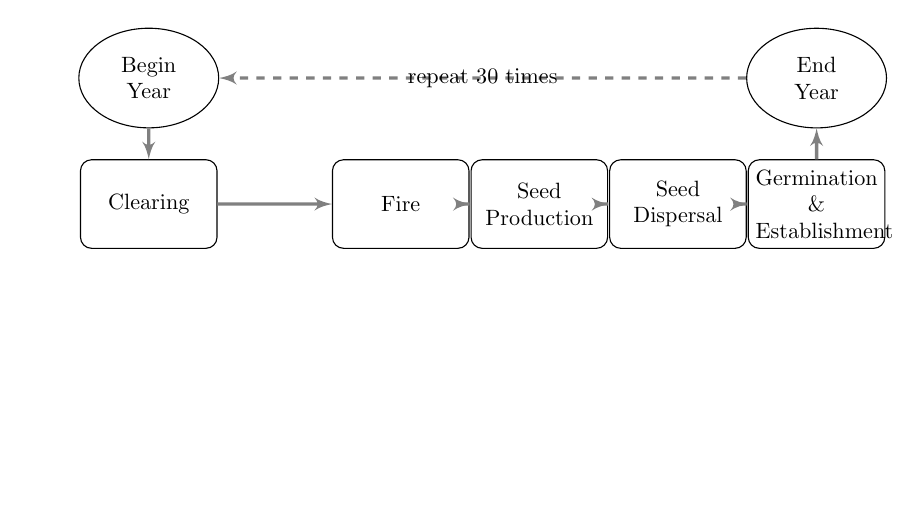
\begin{tikzpicture}[scale=0.8, transform shape]
% Place nodes Overview
    \node [beginend] (beginOverview) {Begin Year};
    \node [block, below of=beginOverview, node distance=2cm] (clear) {Clearing};
    \node [block, right of=clear, node distance=4cm] (fire) {Fire};
    \node [block, right of=fire, node distance=2.2cm] (seedprod) {Seed Production};
    \node [block, right of=seedprod, node distance=2.2cm] (seeddisp) {Seed Dispersal};
    \node [block, right of=seeddisp, node distance=2.2cm] (germest) {Germination \& Establishment};
    \node [beginend, above of=germest, node distance=2cm] (endOverview) {End Year};

% Draw conectors Overview
    \path [line] (beginOverview) -- (clear);
    \path [line] (clear) -- (fire);
    \path [line] (fire) -- (seedprod);
    \path [line] (seedprod) -- (seeddisp);
    \path [line] (seeddisp) -- (germest);
    \path [line] (germest) -- (endOverview);
    \path [line, dashed] (endOverview) -- node {\textcolor{black} {repeat 30 times}} (beginOverview);

% Place nodes Clearing
    \node [subblock, below of=clear, left=0.9cm, below=-1cm, opacity=0] (costs) {Determine costs per cell};
    \node [subblock, below of=costs, node distance=1.7cm, opacity=0] (identify) {Identify area to be cleared};
    
    \node [subblock, below of=clear, right=0.9cm, below=-1cm, opacity=0] (budget) {Save remaining budget};
    \node [subblock, below of=budget, node distance=1.7cm, opacity=0] (clear) {Clear IAPs};

% Draw connectors Clearing
    \path [line, opacity=0] (costs) -- (identify);
    \path [line, opacity=0] (identify) -- (clear);
    \path [line, opacity=0] (clear) -- (budget);

% Place nodes Fire
%    \node [subblock, below of=fire, left=0.9cm, below=-1cm] (fm) {Determine fuel model};
%    \node [subblock, below of=fm, node distance=1.7cm] (ros) {Determine ros};
%    \node [subblock, below of=ros, node distance=1.7cm] (ignrisk) {Determine ignition risk};
    
%    \node [subblock, below of=fire, right=0.9cm, below=-1cm] (burn) {Burn cells};
%    \node [subblock, below of=burn, node distance=1.7cm] (area) {Identify cells to be burned};
%   \node [subblock, below of=area, node distance=1.7cm] (spread) {Calculate temporal and spatial fire spread};

%    \node [subblock, below of=ignrisk, below=-0.3cm, right=0.1cm] (ign) {Determine ignition points};

% Draw connectors Fire
%    \path [line] (fm) -- (ros);
%    \path [line] (ros) -- (ignrisk);
%    \path [line] (ignrisk) -- (ign);
%    \path [line] (ign) -- (spread);
%    \path [line] (spread) -- (area);
%    \path [line] (area) -- (burn);

\end{tikzpicture}

\onslide<2>\scriptsize
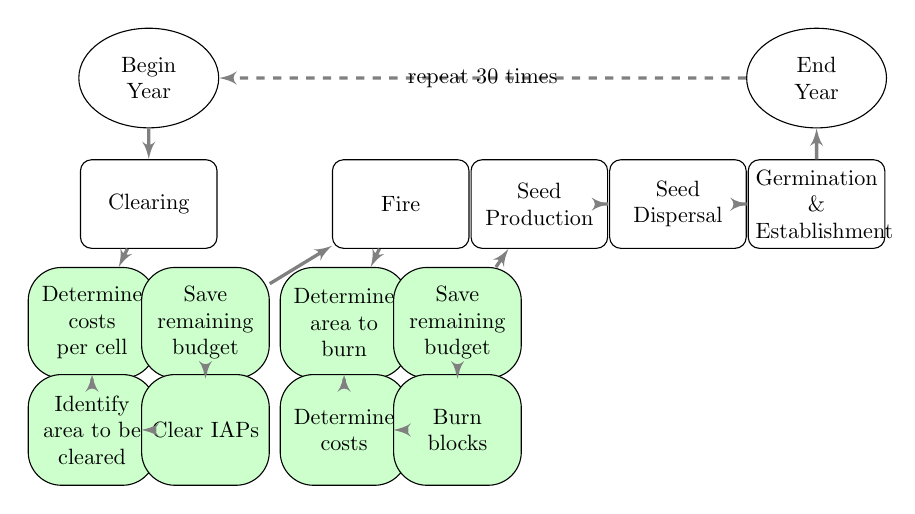
\begin{tikzpicture}[scale=0.8, transform shape]
% Place nodes Overview
    \node [beginend] (beginOverview) {Begin Year};
    \node [block, below of=beginOverview, node distance=2cm] (clear) {Clearing};
    \node [block, right of=clear, node distance=4cm] (fire) {Fire};
    \node [block, right of=fire, node distance=2.2cm] (seedprod) {Seed Production};
    \node [block, right of=seedprod, node distance=2.2cm] (seeddisp) {Seed Dispersal};
    \node [block, right of=seeddisp, node distance=2.2cm] (germest) {Germination \& Establishment};
    \node [beginend, above of=germest, node distance=2cm] (endOverview) {End Year};

% Draw conectors Overview
    \path [line] (beginOverview) -- (clear);
%    \path [line] (clear) -- (fire);
%    \path [line] (fire) -- (seedprod);
    \path [line] (seedprod) -- (seeddisp);
    \path [line] (seeddisp) -- (germest);
    \path [line] (germest) -- (endOverview);
    \path [line, dashed] (endOverview) -- node {\textcolor{black} {repeat 30 times}} (beginOverview);

% Place nodes Clearing
    \node [subblock, below of=clear, left=0.9cm, below=-1cm] (costs) {Determine costs per cell};
    \node [subblock, below of=costs, node distance=1.7cm] (identify) {Identify area to be cleared};
    
    \node [subblock, below of=clear, right=0.9cm, below=-1cm] (budget) {Save remaining budget};
    \node [subblock, below of=budget, node distance=1.7cm] (clearA) {Clear IAPs};

% Draw connectors Clearing
    \path [line] (clear) -- (costs);
    
    \path [line] (costs) -- (identify);
    \path [line] (identify) -- (clearA);
    \path [line] (clearA) -- (budget);

	\path [line] (budget) -- (fire);

% Place nodes Fire
    \node [subblock, below of=fire, left=0.9cm, below=-1cm] (blockF) {Determine area to burn};
    \node [subblock, below of=blockF, node distance=1.7cm] (costF) {Determine costs};
    \node [subblock, below of=fire, right=0.9cm, below=-1cm] (budgetF) {Save remaining budget};
    \node [subblock, below of=budgetF, node distance=1.7cm] (burnF) {Burn blocks};
    
%     \node [subblock, below of=ignrisk, below=-0.3cm, right=0.1cm] (ign) {Determine ignition points};

% Draw connectors Fire
    \path [line] (fire) -- (blockF);

    \path [line] (blockF) -- (costF);
    \path [line] (costF) -- (burnF);
    \path [line] (burnF) -- (budgetF);

    \path [line] (budgetF) -- (seedprod);

\end{tikzpicture}
\end{overprint}

\lyxframeend{}\lyxplainframe{}

\begin{center}
\includegraphics[width=1\textwidth,height=0.95\textheight,keepaspectratio]{MaxCologne-Rohbau_September_2011-3057}
\par\end{center}

{\tiny{� Raimond Spekking / CC-BY-SA-3.0 (via Wikimedia Commons) {[}CC-BY-SA-3.0
(http://creativecommons.org/licenses/by-sa/3.0) or GFDL (http://www.gnu.org/copyleft/fdl.html){]},
via Wikimedia Commons}}{\tiny \par}


\lyxframeend{}\lyxplainframe{}

\begin{center}
\includegraphics[width=1\textwidth,height=1\textheight,keepaspectratio]{warehouse}
\par\end{center}

{\tiny{� http://lerablog.org/business/management/ensure-the-safety-of-your-warehouse/}}{\tiny \par}


\lyxframeend{}\lyxplainframe{}

\begin{center}
\includegraphics[width=1\textwidth,height=1\textheight,keepaspectratio]{trucker2}
\par\end{center}

{\tiny{� http://www.schulen.regensburg.de/\textasciitilde{}tkoe2207/weihnachtsaktion.htm}}{\tiny \par}


\lyxframeend{}\lyxplainframe{}

\begin{center}
\includegraphics[width=1\linewidth,height=1\textheight,keepaspectratio]{packages-2_3}
\par\end{center}

{\tiny{� http://webapp1.wright.edu/housing/addresses.php, edited by
myself}}{\tiny \par}


\lyxframeend{}

}


\lyxframeend{}\section{Optimising in Fynbos}


\lyxframeend{}

{ 
\usebackgroundtemplate{\includegraphics[width=1\paperwidth,height=1\paperheight,keepaspectratio]{Invasions\lyxdot res}}


\lyxframeend{}\lyxplainframe{Optimising in Fynbos}


\lyxframeend{}

}

{ 
\usebackgroundtemplate{\includegraphics[width=1\paperwidth,height=1\paperheight,keepaspectratio]{Invasions\lyxdot res\lyxdot bw}}


\lyxframeend{}\lyxplainframe{Different Funding Scenarios}

\begin{center}
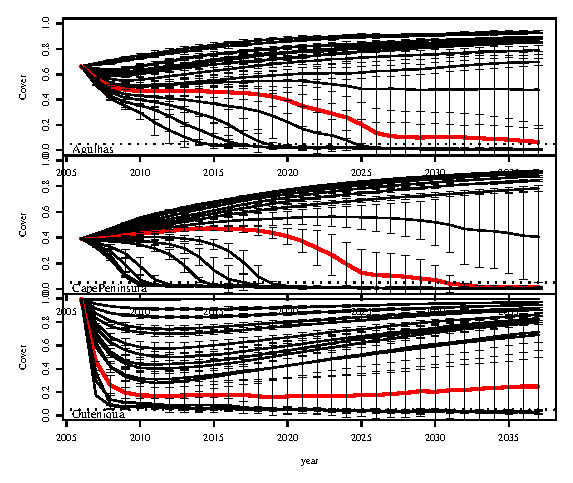
\includegraphics[bb=0bp 0bp 259bp 216bp,scale=0.95]{cover_Krug2010}
\par\end{center}

{\tiny{Krug, R. M., Roura-Pascual, N., \& Richardson, D. M. (2010).
Clearing of invasive alien plants under different budget scenarios:
using a simulation model to test efficiency. Biological Invasions,
12(12), 4099\textendash{}4112. doi:10.1007/s10530-010-9827-3}}{\tiny \par}


\lyxframeend{}\lyxplainframe{Different Management Scenarios}

\selectlanguage{british}%
\begin{tabular}{>{\centering}m{0.5in}|>{\centering}m{0.6in}>{\centering}m{0.6in}>{\centering}m{0.6in}>{\centering}m{0.6in}>{\centering}m{0.6in}}
\selectlanguage{english}%
\selectlanguage{british}%
 & Random & Consensus & Past & Present & Future\tabularnewline
\hline 
Agulhas & \medskip{}
\includegraphics{Agulhas\lyxdot Random\lyxdot Agulhas_new} & \medskip{}
\includegraphics{Agulhas\lyxdot Consensus\lyxdot Agulhas_new} & \medskip{}
\includegraphics{Agulhas\lyxdot Past\lyxdot Agulhas_new} & \medskip{}
\includegraphics{Agulhas\lyxdot Present\lyxdot Agulhas_new} & \medskip{}
\includegraphics{Agulhas\lyxdot Future\lyxdot Agulhas_new}\tabularnewline
Cape Peninsula & \medskip{}
\includegraphics{CapePeninsula\lyxdot Random\lyxdot CapePeninsula_new} & \medskip{}
\includegraphics{CapePeninsula\lyxdot Consensus\lyxdot CapePeninsula_new} & \medskip{}
\includegraphics{CapePeninsula\lyxdot Past\lyxdot CapePeninsula_new} & \medskip{}
\includegraphics{CapePeninsula\lyxdot Present\lyxdot CapePeninsula_new} & \medskip{}
\includegraphics{CapePeninsula\lyxdot Future\lyxdot CapePeninsula_new}\tabularnewline
Outeni-qua & \medskip{}
\includegraphics{Outeniqua\lyxdot Random\lyxdot Outeniqua_new} & \medskip{}
\includegraphics{Outeniqua\lyxdot Consensus\lyxdot Outeniqua_new} & \medskip{}
\includegraphics{Outeniqua\lyxdot Past\lyxdot Outeniqua_new} & \medskip{}
\includegraphics{Outeniqua\lyxdot Present\lyxdot Outeniqua_new} & \medskip{}
\includegraphics{Outeniqua\lyxdot Future\lyxdot Outeniqua_new}\tabularnewline
\end{tabular}

\selectlanguage{english}%

\lyxframeend{}

}


\lyxframeend{}\section{How to make it accessible}


\lyxframeend{}

{ 
\usebackgroundtemplate{

\includegraphics[width=1\paperwidth,height=1\paperheight]{presentation-cloud-computing_bkg}

}


\lyxframeend{}\lyxplainframe{}

\begin{center}
\includegraphics[width=1\textwidth,height=1\textheight]{presentation-cloud-computing_2}
\par\end{center}

\begin{center}
{\tiny{� http://www.itresearch.fr/industrialisation-informatique/
edited by myself}}
\par\end{center}{\tiny \par}


\lyxframeend{}\lyxframe{[plain,allowframebreaks]User Interface}

\begin{center}
\includegraphics[width=1\textwidth,height=1\textheight,keepaspectratio]{gruber}
\par\end{center}

\begin{center}
{\tiny{� http://uxmag.com/articles/the-dirtiest-word-in-ux-complexity}}
\par\end{center}{\tiny \par}

\pagebreak{}

\includegraphics[bb=0bp 0bp 232bp 259bp,clip,scale=0.65]{blender}

{\tiny{� http://uxmag.com/articles/the-dirtiest-word-in-ux-complexity}}{\tiny \par}

\pagebreak{}

\includegraphics[scale=0.65]{blender}

{\tiny{� http://uxmag.com/articles/the-dirtiest-word-in-ux-complexity}}{\tiny \par}


\lyxframeend{}\lyxframe{Where we are}
\begin{enumerate}
\item Developing generic spread model
\item Parametrize spread model
\item Identify ecosystem service models
\item Develop simple interface
\end{enumerate}

\lyxframeend{}\lyxplainframe{Bringing Science and management together?}


\pause{}

\begin{center}
\includegraphics[clip,width=1\paperwidth,height=0.85\paperheight,keepaspectratio]{rosie_the_riveter}
\par\end{center}


\lyxframeend{}\lyxframe{Acknowledgements}
\begin{itemize}
\item This project is financed by Ezemvelo KZN Wildlife.
\item Conference attendance financed by the Centre of Excellence for Invasion
Biology, Stellenbosch University
\item Software used (OpenSource only)

\begin{itemize}
\item Presentation: 

\begin{itemize}
\item \LyX{} \url{http://www.lyx.org}
\item \LaTeX{} \url{http://www.latex-project.org/}
\item Beamer \url{https://bitbucket.org/rivanvx/beamer/wiki/Home}
\end{itemize}
\item Charts

\begin{itemize}
\item PlantUML \url{http://http://plantuml.sourceforge.net}
\end{itemize}
\item and others
\end{itemize}
\end{itemize}

\lyxframeend{}

}


\lyxframeend{}
\end{document}
